\documentclass{standalone}

\usepackage{tikz}
\usepackage{tkz-graph}
\usetikzlibrary{decorations.pathreplacing}
\usetikzlibrary{matrix}
\thispagestyle{empty}
\begin{document}
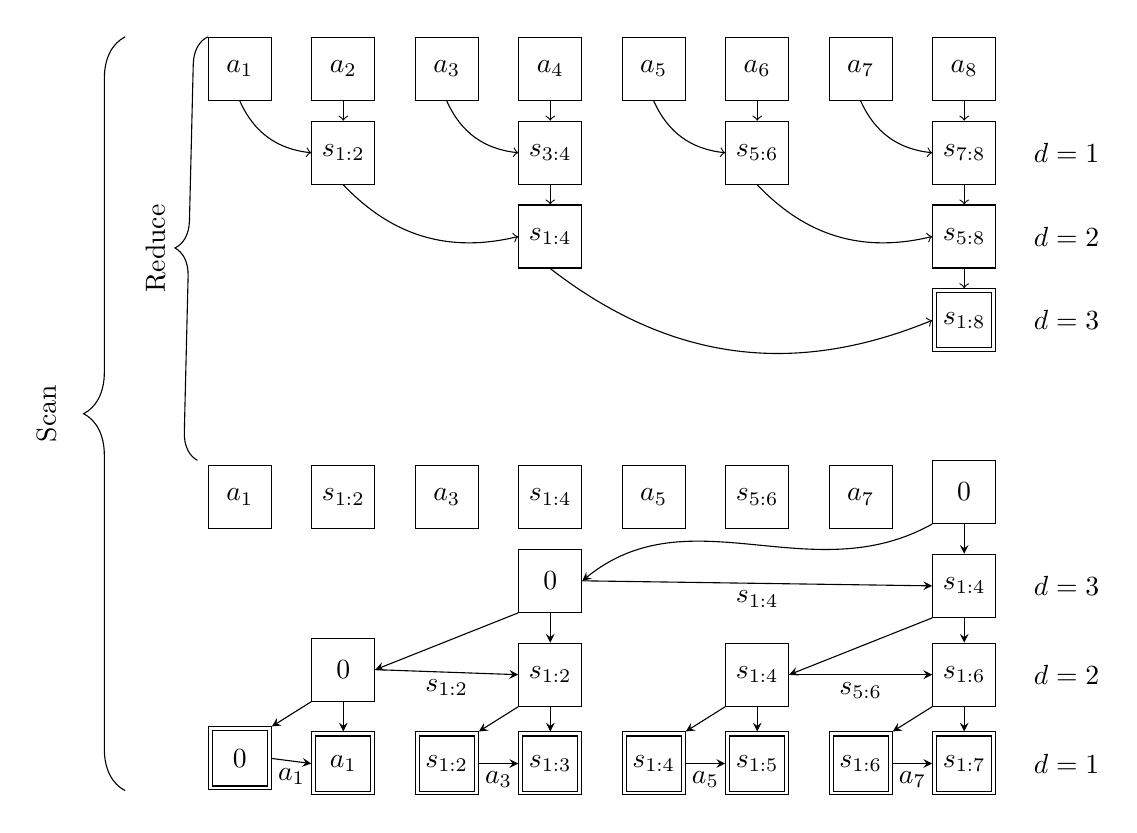
\begin{tikzpicture}[scale=1.5]

%\newcommand{\mybox}[1]{\node[rectangle, draw]{#1};}
%\newcommand{\myboxd}[1]{\node[rectangle, dashed, draw]{#1};}
\matrix(u)[matrix of nodes, column sep=0.5cm,row sep=0.25cm,
			 nodes={draw, minimum width=.8cm, minimum height=.8cm}]
{%
$a_1$ & $a_2$ & $a_3$ & $a_4$ & $a_5$ & $a_6$ & $a_7$ & $a_8$\\
& $s_{1:2}$ & & $s_{3:4}$ & & $s_{5:6}$ & & $s_{7:8}$\\
&&& $s_{1:4}$ & & & & $s_{5:8}$\\
&&&&&&& $s_{1:8}$\\
};

\node[draw=none, fill=none, minimum width=.8cm, minimum height=.8cm, xshift=1.3cm] at (u-2-8.center) {$d=1$};
\node[draw=none, fill=none, minimum width=.8cm, minimum height=.8cm, xshift=1.3cm] at (u-3-8.center) {$d=2$};
\node[draw=none, fill=none, minimum width=.8cm, minimum height=.8cm, xshift=1.3cm] at (u-4-8.center) {$d=3$};
\draw[->, bend right](u-1-1.south) to (u-2-2.west);
\draw[->, bend right](u-1-3.south) to (u-2-4.west);
\draw[->, bend right](u-1-5.south) to (u-2-6.west);
\draw[->, bend right](u-1-7.south) to (u-2-8.west);
\draw[->](u-1-2.south) to (u-2-2.north);
\draw[->](u-1-4.south) to (u-2-4.north);
\draw[->](u-1-6.south) to (u-2-6.north);
\draw[->](u-1-8.south) to (u-2-8.north);

\draw[->, bend right](u-2-2.south) to (u-3-4.west);
\draw[->, bend right](u-2-6.south) to (u-3-8.west);
\draw[->](u-2-4.south) to (u-3-4.north);
\draw[->](u-2-8.south) to (u-3-8.north);

\draw[->, bend right](u-3-4.south) to (u-4-8.west);
\draw[->](u-3-8.south) to (u-4-8.north);
\node[rectangle, minimum width=.7cm, minimum height=.7cm, draw] at (u-4-8){};

\draw [decorate,decoration={brace,amplitude=10pt},xshift=0,yshift=.25cm]
(-3.425,-2.5) -- (u-1-1.north west) node [black,midway,xshift=-0.6cm,rotate=90] {Reduce};


\matrix(d)[matrix of nodes, column sep=0.5cm,row sep=0.25cm,
			 nodes={draw, minimum width=.8cm, minimum height=.8cm}, yshift=-5.5cm]
{
$a_1$ & $s_{1:2}$ & $a_3$ & $s_{1:4}$ & $a_5$ & $s_{5:6}$ & $a_7$ & $0$\\
&&& $0$ & & & & $s_{1:4}$\\
&$0$ & & $s_{1:2}$ & & $s_{1:4}$ & & $s_{1:6}$\\
$0$& $a_1$ & $s_{1:2}$ & $s_{1:3}$ & $s_{1:4}$ & $s_{1:5}$ & $s_{1:6}$ & $s_{1:7}$\\
};
\node[rectangle, minimum width=.8cm, minimum height=.8cm, draw] at (d-1-8){};

\node[draw=none, fill=none, minimum width=.8cm, minimum height=.8cm, xshift=1.3cm] at (d-2-8.center) {$d=3$};
\node[draw=none, fill=none, minimum width=.8cm, minimum height=.8cm, xshift=1.3cm] at (d-3-8.center) {$d=2$};
\node[draw=none, fill=none, minimum width=.8cm, minimum height=.8cm, xshift=1.3cm] at (d-4-8.center) {$d=1$};


%left child inherits root
\draw[->, >=stealth, bend left=10](d-1-8.south west) to[out=20, in=210] (d-2-4.east);
\draw[->, >=stealth](d-2-8.south west) to (d-3-6.east);
\draw[->, >=stealth](d-2-4.south west) to (d-3-2.east);
\draw[->, >=stealth](d-3-8.south west) to (d-4-7.north east);
\draw[->, >=stealth](d-3-6.south west) to (d-4-5.north east);
\draw[->, >=stealth](d-3-4.south west) to (d-4-3.north east);
\draw[->, >=stealth](d-3-2.south west) to (d-4-1.north east);

%left child passes up its value
\draw[->, >=stealth, bend right=10](d-2-4.east) -- (d-2-8.west) node [black,midway,yshift=-.2cm]{$s_{1:4}$};
\draw[->, >=stealth, bend right=10](d-3-6.east) -- (d-3-8.west)  node [black,midway,yshift=-.2cm]{$s_{5:6}$};
\draw[->, >=stealth, bend right=10](d-3-2.east) -- (d-3-4.west) node [black,midway,yshift=-.2cm]{$s_{1:2}$};
\draw[->, >=stealth, bend right=10](d-4-7.east) -- (d-4-8.west) node [black,midway,yshift=-.2cm]{$a_7$};
\draw[->, >=stealth, bend right=10](d-4-5.east) -- (d-4-6.west) node [black,midway,yshift=-.2cm]{$a_5$};
\draw[->, >=stealth, bend right=10](d-4-3.east) -- (d-4-4.west) node [black,midway,yshift=-.2cm]{$a_3$};
\draw[->, >=stealth, bend right=10](d-4-1.east) -- (d-4-2.west) node [black,midway,yshift=-.2cm]{$a_1$};

%root accumulates
\draw[->, >=stealth](d-1-8.south) to (d-2-8.north);
\draw[->, >=stealth](d-2-8.south) to (d-3-8.north);
\draw[->, >=stealth](d-2-4.south) to (d-3-4.north);
\draw[->, >=stealth](d-3-8.south) to (d-4-8.north);
\draw[->, >=stealth](d-3-6.south) to (d-4-6.north);
\draw[->, >=stealth](d-3-4.south) to (d-4-4.north);
\draw[->, >=stealth](d-3-2.south) to (d-4-2.north);
%\draw[<->, dashed, bend left] (d-1-1.north) to (d-1-2.north);
%\draw[->] (d-1-2.south) -- (d-2-2.north);

%identify result
\node[rectangle, minimum width=.7cm, minimum height=.7cm, draw] at (d-4-8){};
\node[rectangle, minimum width=.7cm, minimum height=.7cm, draw] at (d-4-7){};
\node[rectangle, minimum width=.7cm, minimum height=.7cm, draw] at (d-4-6){};
\node[rectangle, minimum width=.7cm, minimum height=.7cm, draw] at (d-4-5){};
\node[rectangle, minimum width=.7cm, minimum height=.7cm, draw] at (d-4-4){};
\node[rectangle, minimum width=.7cm, minimum height=.7cm, draw] at (d-4-3){};
\node[rectangle, minimum width=.7cm, minimum height=.7cm, draw] at (d-4-2){};
\node[rectangle, minimum width=.7cm, minimum height=.7cm, draw] at (d-4-1){};
%\node[rotate=90,xshift=1.3cm,yshift=.5cm] at (d-4-1.north west) {downsweep};
\draw [decorate,decoration={brace,amplitude=15pt},yshift=.25cm]
([xshift=-.7cm]d-4-1.south west) -- ([xshift=-.7cm]u-1-1.north west) node [black,midway,xshift=-1cm,rotate=90] {Scan};
%\draw[gray,step=0.25] (-5, -5.25) grid (4.5, 1.5);
%\clip (-5, -5.25) rectangle (4.5, 1.5);
\clip (-1,-1) rectangle (1,1);
\end{tikzpicture}

\end{document}